\subsection{Additional Run Time
  Benchmarks}\label{cockpit::app:run-time-benchmarks}

\subsubsection{Individual Instrument
  Overhead}\label{cockpit::app:benchmark-instruments}
To estimate the computational overhead for individual instruments, we run
\cockpit with that instrument for $32$ iterations, tracking at every step.
Training proceeds with the default batch size specified by the \deepobs problem
and uses \sgd with learning rate $10^{-3}$. We measure the time between
iterations $1$ and $32$, and average for the overhead per step. Every such
estimate is repeated over $10$ random seeds to obtain mean and error bars as
reported in \Cref{cockpit::fig:benchmark-instruments}.

Note that this protocol does \textit{not} include initial overhead for setting
up data loading and also does \textit{not} include the time for evaluating
train/test loss on a larger dataset, which is usually done by practitioners.
Hence, we even expect the shown overheads to be smaller in a conventional
training loop which includes the above steps.

\subsubsection{Individual Overhead on GPU Versus CPU}

\Cref{cockpit::fig:app_benchmark_instruments_cuda} and
\Cref{cockpit::fig:app_benchmark_instruments_cpu} show the individual overhead
for four different \deepobs problems on GPU and CPU, respectively. The left part
of \Cref{cockpit::fig:app_benchmark_instruments_cuda} (c) corresponds to
\Cref{cockpit::fig:benchmark-instruments}. Right panels show the expensive
quantities, which we omitted in the main text as they were expected to be
expensive due to their computational work (\inlinecode{HessMaxEV}) or
bottlenecks in the implementation (\inlinecode{GradHist2d}, see
\Cref{cockpit::app:histograms} for details). We see that they are in many cases
equally or more expensive than computing all other instruments. Another expected
feature of the GPU-to-CPU comparison is that parallelism on the CPU is
significantly less pronounced. Hence, we observe an increased overhead for all
quantities that contain non-linear transformations and contractions of the
high-dimensional individual gradients, or require additional backpropagations
(curvature).

\captionsetup[subfigure]{justification=justified,singlelinecheck=false}

\begin{figure*}[p]
  \vfill
  \begin{subfigure}[t]{\linewidth}
    \caption{Computational overhead for \mnist \MNISTNET (GPU)}
    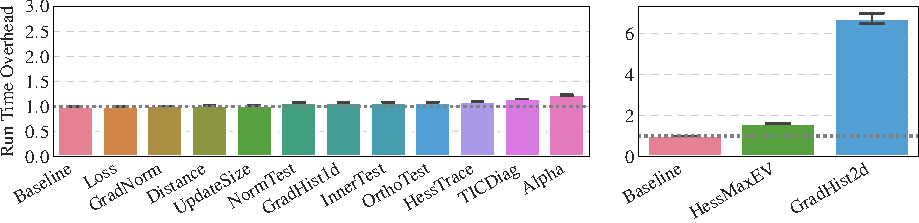
\includegraphics{../repos/cockpit-paper/fig/01_benchmark/output/fig_individual/benchmark_combined_mnist_logreg_cuda_thesis-wide}
    \label{cockpit::fig:app_benchmark_instruments_cuda-mnist_logreg}
  \end{subfigure}
  \vfill
  \begin{subfigure}[t]{\linewidth}
    \caption{Computational overhead for \mnist \mlp (GPU)}
    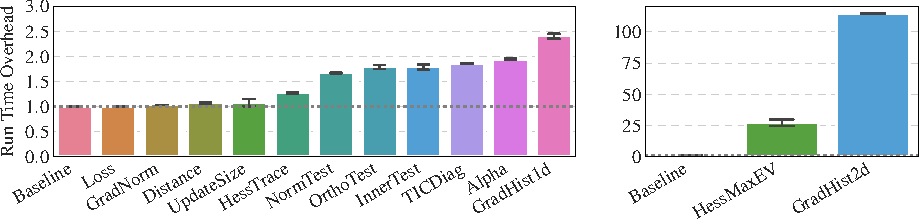
\includegraphics{../repos/cockpit-paper/fig/01_benchmark/output/fig_individual/benchmark_combined_mnist_mlp_cuda_thesis-wide}
    \label{cockpit::fig:app_benchmark_instruments_cuda-mnist_mlp}
  \end{subfigure}
  \vfill
  \begin{subfigure}[t]{\linewidth}
    \caption{Computational overhead for \cifarten \threecthreed (GPU)}
    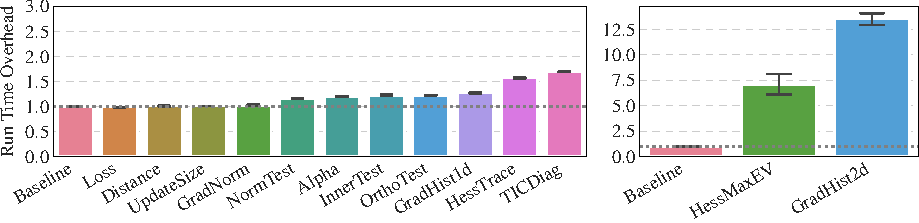
\includegraphics{../repos/cockpit-paper/fig/01_benchmark/output/fig_individual/benchmark_combined_cifar10_3c3d_cuda_thesis-wide}
    \label{cockpit::fig:app_benchmark_instruments_cuda-cifar10}
  \end{subfigure}
  \vfill
  \begin{subfigure}[t]{\linewidth}
    \caption{Computational overhead for \fmnist \twoctwod (GPU)}
    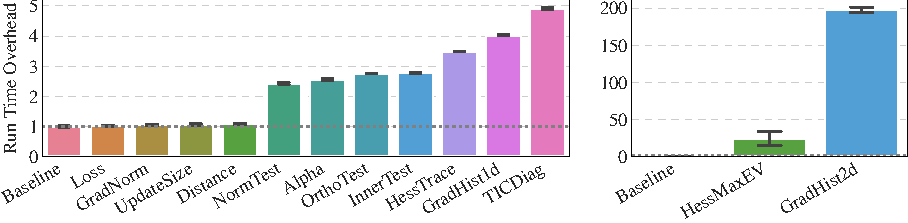
\includegraphics{../repos/cockpit-paper/fig/01_benchmark/output/fig_individual/benchmark_combined_fmnist_2c2d_cuda_thesis-wide}
    \label{cockpit::fig:app_benchmark_instruments_cuda-fmnist}
  \end{subfigure}
  \vfill
  \caption{\textbf{Individual overhead of \cockpittitle's instruments on GPU for
      four different problems.} All run times are shown as multiples of the
    \emph{baseline} without tracking. Expensive quantities are displayed in
    separate panels on the right. Experimental details in the text.}
  \label{cockpit::fig:app_benchmark_instruments_cuda}
\end{figure*}

\captionsetup[subfigure]{justification=centering, singlelinecheck=true}

%%% Local Variables:
%%% mode: latex
%%% TeX-master: "../../../thesis"
%%% End:


\captionsetup[subfigure]{justification=justified,singlelinecheck=false}

\begin{figure*}[p]
  \vfill
  \begin{subfigure}[t]{\linewidth}
    \caption{Computational overhead for \mnist \MNISTNET (CPU)}
    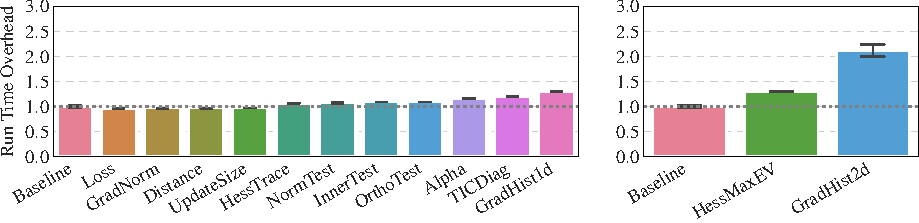
\includegraphics{../repos/cockpit-paper/fig/01_benchmark/output/fig_individual/benchmark_combined_mnist_logreg_cpu_thesis-wide}
    \label{cockpit::fig:app_benchmark_instruments_cpu-mnist_logreg}
  \end{subfigure}
  \vfill
  \begin{subfigure}[t]{\linewidth}
    \caption{Computational overhead for \mnist \mlp (CPU)}
    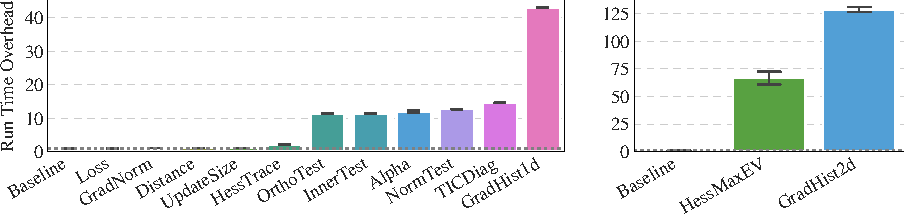
\includegraphics{../repos/cockpit-paper/fig/01_benchmark/output/fig_individual/benchmark_combined_mnist_mlp_cpu_thesis-wide}
    \label{cockpit::fig:app_benchmark_instruments_cpu-mnist_mlp}
  \end{subfigure}
  \vfill
  \begin{subfigure}[t]{\linewidth}
    \caption{Computational overhead for \cifarten \threecthreed (CPU)}
    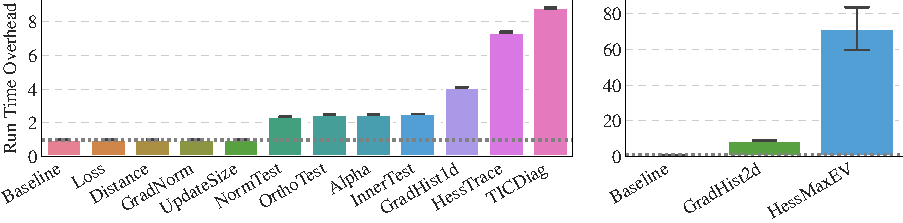
\includegraphics{../repos/cockpit-paper/fig/01_benchmark/output/fig_individual/benchmark_combined_cifar10_3c3d_cpu_thesis-wide}
    \label{cockpit::fig:app_benchmark_instruments_cpu-cifar10}
  \end{subfigure}
  \vfill
  \begin{subfigure}[t]{\linewidth}
    \caption{Computational overhead for \fmnist \twoctwod (CPU)}
    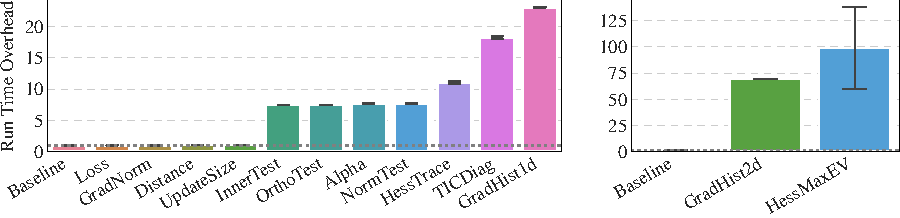
\includegraphics{../repos/cockpit-paper/fig/01_benchmark/output/fig_individual/benchmark_combined_fmnist_2c2d_cpu_thesis-wide}
    \label{cockpit::fig:app_benchmark_instruments_cpu-fmnist}
  \end{subfigure}
  \vfill
  \caption{\textbf{Individual overhead of \cockpittitle's instruments on CPU for
      four different problems.} All run times are shown as multiples of the
    \emph{baseline} without tracking. Expensive quantities are displayed in
    separate panels on the right. Experimental details in the text.}
  \label{cockpit::fig:app_benchmark_instruments_cpu}
\end{figure*}

\captionsetup[subfigure]{justification=centering, singlelinecheck=true}

%%% Local Variables:
%%% mode: latex
%%% TeX-master: "../../../thesis"
%%% End:


%%% Local Variables:
%%% mode: latex
%%% TeX-master: "../thesis"
%%% End:
